\documentclass{exercise}

\institute{Lehr- und Forschungsgebiet Kontinuumsmechanik}
\title{Übung 11}
\author{Joshua Feld, 406718}
\course{Mechanik verformbarer Körper}
\professor{Itskov}
\semester{Sommersemester 2022}
\program{CES (Bachelor)}

\begin{document}
    \maketitle
    
    
    \section*{Aufgabe 1}
    
    \begin{problem}
        Ein Kragbalken mit einem um den Winkel \(\alpha\) schiefgestellten Querschnitt wurd durch ein Moment \(M\) belastet.
        Der Balken habe ein Rechteckprofil mit Höhe \(h\) und Breite \(b\).
        Berechnen Sie die maximale Biegespannung.
        
        Gegeben: \(h = 1,5\sis{\centi\meter}\), \(b = 0,5\sis{\centi\meter}\), \(M = 25\sis{\newton\meter}\), \(\alpha = 30^\circ\)
    \end{problem}
    
    \subsection*{Lösung}
    Die Hauptflächenträgheitsmomente lassen sich einfach zu
    \[
        I_{y'} = \frac{bh^3}{12} = 15,625 \cdot 10^{-3}\sis{\centi\meter\tothe{4}}, \quad I_{z'} = \frac{b^3 h}{12} = 140,625 \cdot 10^{-3}\sis{\centi\meter\tothe{4}}, \quad I_{y'z'} = 0\sis{\centi\meter\tothe{4}}
    \]
    berechnen.
    Die Zerlegung des Biegemoments im Hauptachsenanteile ergibt
    \[
        M_{y'} = M\sin\alpha = 12,5\sis{\newton\meter}, \quad M_{z'} = M\cos\alpha = 21,7\sis{\newton\meter}.
    \]
    Die Spannung ist an den Ecken am größten.
    Mit der Gleichung für die Biegespannung
    \[
        \sigma_b\parentheses*{y', z'} = \frac{M_{y'}}{I_{y'}}z' - \frac{M_{z'}}{I_{z'}}y'
    \]
    folgt somit
    \[
        \sigma_{b, \text{max}} = \sigma_b\parentheses*{-\frac{h}{2}, \frac{b}{2}} = 315,47\sis{\newton\per\milli\meter\squared}.
    \]
    
    
    \section*{Aufgabe 2}
    
    \begin{problem}
        Für einen Kraftträger der Länge \(l\) mit konstanter Biegesteifigkeit \(EI\) sind jeweils für Fall 1 (endseitige Kraft \(F\)) und Fall 2 (endseitiges Biegemoment \(M_0\)) die größte Drehbiegung und der größte Neigungswinkel zu ermitteln.
        
        Gegeben: \(E\), \(I\), \(l\), \(F\), \(M_0\)
    \end{problem}
    
    \subsection*{Lösung}
    \begin{itemize}
        \item Fall 1: Für das Biegemoment in Abhängigkeit von \(x\) ergibt sich aus dem Momentengleichgewicht
        \[
            M\parentheses*{x} = -F\parentheses*{l - x}.
        \]
        Aus der Definition der Biegelinie
        \[
            w''\parentheses*{x} = -\frac{M\parentheses*{x}}{EI}
        \]
        folgt durch zweimaliges integrieren
        \begin{align*}
            EIw''\parentheses*{x} &= -Fx + Fl,\\
            EIw'\parentheses*{x} &= -\frac{1}{2}Fx^2 + Flx + c_1,\\
            EIw\parentheses*{x} &= -\frac{1}{6}Fx^3 + \frac{1}{2}Flx^2 + c_1 x + c_2.
        \end{align*}
        Durch die Randbedingungen \(w\parentheses*{0} = 0\) (keine Durchbiegung in der Einspannung) und \(w'\parentheses*{0} = 0\) (kein Knick in der Einspannung) folgt für die Integrationskonstanten
        \[
            c_1 = 0, \quad c_2 = 0
        \]
        und somit
        \begin{align*}
            EIw''\parentheses*{x} &= -Fx + Fl,\\
            EIw'\parentheses*{x} &= -\frac{1}{2}Fx^2 + Flx,\\
            EIw\parentheses*{x} &= -\frac{1}{6}Fx^3 + \frac{1}{2}Flx^2.
        \end{align*}
        Die maximale Durchbiegung und der maximale Neigungswinkel befinden sich am Ende des Trägers
        \[
            w\parentheses*{l} = \frac{Fl^3}{3EI}, \quad w'\parentheses*{l} = \frac{Fl^2}{2EI}.
        \]
        \item Fall 2: Für das Biegemoment in Abhängigkeit von \(x\) ergibt sich aus dem Momentengleichgewicht
        \[
            M\parentheses*{x} = -M_0.
        \]
        Aus der Definition der Biegelinie
        \[
            w''\parentheses*{x} = -\frac{M\parentheses*{x}}{EI}
        \]
        folgt durch zweimaliges Integrieren
        \begin{align*}
            EIw''\parentheses*{x} &= M_0,\\
            EIw'\parentheses*{x} &= M_0 x + c_1,\\
            EIw\parentheses*{x} &= \frac{1}{2}M_0 x^2 + c_1 x + c_2.
        \end{align*}
        Durch die Randbedingungen \(w\parentheses*{0} = 0\) (keine Durchbiegung in der Einspannung) und \(w'\parentheses*{0} = 0\) (kein Knick in der Einspannung) folgt für die Integrationskonstanten
        \[
            c_1 = 0, \quad c_2 = 0
        \]
        und somit
        \begin{align*}
            EIw''\parentheses*{x} &= M_0,\\
            EIw'\parentheses*{x} &= M_0 x,\\
            EIw\parentheses*{x} &= \frac{1}{2}M_0 x^2.
        \end{align*}
        Die maximale Durchbiegung und der maximale Neigungswinkel befinden sich am Ende des Trägers
        \[
            w\parentheses*{l} = \frac{M_0 l^2}{2EI}, \quad w'\parentheses*{l} = \frac{M_0 l}{EI}.
        \]
    \end{itemize}
    
    
    \section*{Aufgabe 3}
    
    \begin{problem}
        Für den Einfeldträger mit konstanter Biegesteifigkeit \(EI\) sind zu berechnen
        \begin{enumerate}
            \item die Gleichung der Biegelinie,
            \item die Gleichung des Neigungswinkel,
            \item die Durchbiegung in Trägermitte und
            \item die Neigungswinkel der Biegelinie in den Lagern.
        \end{enumerate}
        \begin{center}
            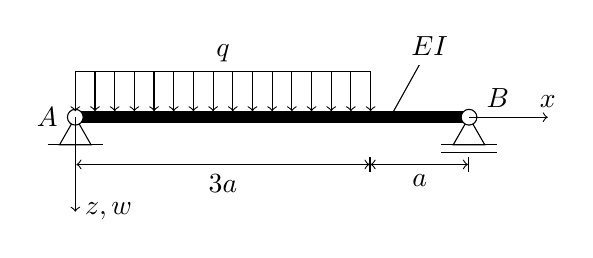
\begin{tikzpicture}
                \draw (-.2,-.25) -- (0,.1) -- (.2,-.25) -- cycle;
                \draw (-.35,-.25) -- (.35,-.25);
                \draw (4.8,-.25) -- (5,.1) -- (5.2,-.25) -- cycle;
                \draw (4.65,-.25) -- (5.35,-.25);
                \draw (4.65,-.35) -- (5.35,-.35);
                \fill (0,.025) rectangle (5,.175);
                \draw[fill=white] (0,.1) circle (1mm);
                \draw[fill=white] (5,.1) circle (1mm);
                \node[anchor=east] at (-.1,.1) {\(A\)};
                \node[anchor=south west] at (5.1,.1) {\(B\)};
                \draw[|<->|] (0,-.5) -- (3.75,-.5) node[midway,below] {\(3a\)};
                \draw[<->|] (3.75,-.5) -- (5,-.5) node[midway,below] {\(a\)};
                \draw[->] (0,.1) -- (0,-1.1) node[right] {\(z, w\)};
                \draw[->] (5,.1) -- (6,.1) node[above] {\(x\)};
                \draw (4,.1) -- (4.5,1) node[fill=white] {\(EI\)};
                \draw (0,.675) -- (3.75,.675) node[midway,above] {\(q\)};
                \foreach \i in {0,.25,...,3.75}
                {
                    \draw[->] (\i,.675) -- (\i,.175);
                }
            \end{tikzpicture}
        \end{center}
        Gegeben: \(E\), \(I\), \(a\), \(q\)
    \end{problem}
    
    \subsection*{Lösung}
    \begin{enumerate}
        \item[a), b)]
        \begin{align*}
            q\parentheses*{x} &= q - q\angles*{x - 3a}^0,\\
            Q\parentheses*{x} &= -qx + q\angles*{x - 3a}^1 + c_1,\\
            M\parentheses*{x} &= -\frac{1}{2}qx^2 + \frac{1}{2}q\angles*{x - 3a}^2 + c_1 x + c_2,\\
            w''\parentheses*{x}EI &= \frac{1}{2}qx^2 - \frac{1}{2}q\angles*{x - 3a}^2 - c_1 x - c_2,\\
            w'\parentheses*{x}EI &= \frac{1}{6}qx^3 - \frac{1}{6}q\angles*{x - 3a}^3 - \frac{1}{2}c_1 x^2 - c_2 x + c_3,\\
            w\parentheses*{x}EI &= \frac{1}{24}qx^4 - \frac{1}{24}q\angles*{x - 3a}^4 - \frac{1}{6}c_1 x^3 - \frac{1}{2}c_2 x^2 + c_3 x + c_4.
        \end{align*}
        Mit den Randbedingungen
        \[
            M\parentheses*{0} = 0, \quad M\parentheses*{4a} = 0, \quad w\parentheses*{0} = 0, \quad w\parentheses*{4a} = 0
        \]
        folgt für die Integrationskonstanten
        \[
            c_1 = \frac{15}{8}qa, \quad c_2 = 0, \quad c_3 = \frac{75}{32}qa^3, \quad c_4 = 0
        \]
        und somit schlussendlich
        \begin{align*}
            q\parentheses*{x} &= q - q\angles*{x - 3a}^0,\\
            Q\parentheses*{x} &= -qx + q\angles*{x - 3a}^1 + \frac{15}{8}qa,\\
            M\parentheses*{x} &= -\frac{1}{2}qx^2 + \frac{1}{2}q\angles*{x - 3a}^2 + \frac{15}{8}qax,\\
            w''\parentheses*{x}EI &= \frac{1}{2}qx^2 - \frac{1}{2}q\angles*{x - 3a}^2 - \frac{15}{8}qax,\\
            w'\parentheses*{x}EI &= \frac{1}{6}qx^3 - \frac{1}{6}q\angles*{x - 3a}^3 - \frac{15}{16}qax^2 + \frac{75}{32}qa^3,\\
            w\parentheses*{x}EI &= \frac{1}{24}qx^4 - \frac{1}{24}q\angles*{x - 3a}^4 - \frac{5}{16}qax^3 + \frac{75}{32}qa^3 x.
        \end{align*}
        \item[c)]
        \[
            w\parentheses*{2a} = \frac{1}{EI}\parentheses*{\frac{2}{3}qa^4 - \frac{5}{2}qa^4 + \frac{75}{16}qa^4} = \frac{137}{48}\frac{qa^4}{EI}.
        \]
        \item[d)]
        \[
            w'\parentheses*{0} = \frac{1}{EI}\frac{75}{32}qa^3 = \frac{75}{32}\frac{qa^3}{EI}, \quad w'\parentheses*{4a} = \frac{1}{EI}\parentheses*{\frac{32}{3}qa^3 - \frac{1}{6}qa^3 - 15qa^3 + \frac{75}{32}qa^3} = -\frac{69}{32}\frac{qa^3}{EI}.
        \]
    \end{enumerate}


    \section*{Aufgabe 4}

    \begin{problem}
        Ein Träger mit konstanter Biegesteifigkeit \(EI\) ist in der angegebenen Weise gelagert und belastet.
        Berechnen Sie mithilfe der Biegelinie die Lagerreaktionen.
        \begin{center}
            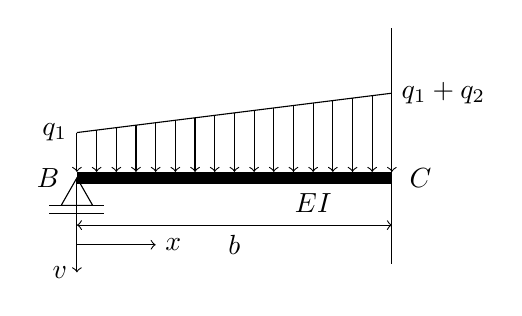
\begin{tikzpicture}
                \draw (-.2,-.25) -- (0,.1) -- (.2,-.25) -- cycle;
                \draw (-.35,-.25) -- (.35,-.25);
                \draw (-.35,-.35) -- (.35,-.35);
                \fill (0,.025) rectangle (4,.175);
                \node[anchor=east] at (-.1,.1) {\(B\)};
                \node[anchor=west] at (4.1,.1) {\(C\)};
                \draw[<->] (0,-.5) -- (4,-.5) node[midway,below] {\(b\)};
                \draw[->] (0,.1) -- (0,-1.1) node[left] {\(v\)};
                \draw[->] (0,-.75) -- (1,-.75) node[right] {\(x\)};
                \node[anchor=north] at (3,0.025) {\(EI\)};
                \draw (0,.675) node[left] {\(q_1\)} -- (4,1.175) node[right] {\(q_1 + q_2\)};
                \foreach \i in {0,.25,...,4}
                {
                    \draw[->] (\i,.675+\i/8) -- (\i,.175);
                }
                \draw (4,2) -- (4,-1);
            \end{tikzpicture}
        \end{center}
        Gegeben: \(q_1\), \(q_2\), \(b\), \(E\), \(I\)
    \end{problem}

    \subsection*{Lösung}
    \begin{align*}
        q\parentheses*{x} &= \frac{q_2}{b}x + q_1,\\
        Q\parentheses*{x} &= -\frac{1}{2}\frac{q_2}{b}x^2 - q_1 x + c_1,\\
        M\parentheses*{x} &= -\frac{1}{6}\frac{q_2}{b}x^3 - \frac{1}{2}q_1 x^2 + c_1 x + c_2,\\
        w''\parentheses*{x}EI &= \frac{1}{6}\frac{q_2}{b}x^3 + \frac{1}{2}q_1 x^2 - c_1 x - c_2,\\
        w'\parentheses*{x}EI &= \frac{1}{24}\frac{q_2}{b}x^4 + \frac{1}{6}q_1 x^3 - \frac{1}{2}c_1 x^2 - c_2 x + c_3,\\
        w\parentheses*{x}EI &= \frac{1}{120}\frac{q_2}{b}x^5 + \frac{1}{24}q_1 x^4 - \frac{1}{6}c_1 x^3 - \frac{1}{2}c_2 x^2 + c_3 x + c_4.
    \end{align*}
    Mit den Randbedingungen
    \[
        M\parentheses*{0} = 0, \quad w\parentheses*{0} = 0, \quad w\parentheses*{b} = 0, \quad w'\parentheses*{b} = 0
    \]
    folgt für die Integrationskonstanten
    \[
        c_1 = \parentheses*{\frac{3}{8}q_1 + \frac{1}{10}q_2}b, \quad c_2 = 0, \quad c_3 = \parentheses*{\frac{1}{48}q_1 + \frac{1}{120}q_2}b^3, \quad c_4 = 0
    \]
    und somit schlussendlich
    \begin{align*}
        q\parentheses*{x} &= \frac{q_2}{b}x + q_1,\\
        Q\parentheses*{x} &= -\frac{1}{2}\frac{q_2}{b}x^2 - q_1 x + \parentheses*{\frac{3}{8}q_1 + \frac{1}{10}q_2}b,\\
        M\parentheses*{x} &= -\frac{1}{6}\frac{q_2}{b}x^3 - \frac{1}{2}q_1 x^2 + \parentheses*{\frac{3}{8}q_1 + \frac{1}{10}q_2}bx,\\
        w''\parentheses*{x}EI &= \frac{1}{6}\frac{q_2}{b}x^3 + \frac{1}{2}q_1 x^2 - \parentheses*{\frac{3}{8}q_1 + \frac{1}{10}q_2}bx,\\
        w'\parentheses*{x}EI &= \frac{1}{24}\frac{q_2}{b}x^4 + \frac{1}{6}q_1 x^3 - \parentheses*{\frac{3}{16}q_1 + \frac{1}{20}q_2}bx^2 + \parentheses*{\frac{1}{48}q_1 + \frac{1}{120}q_2}b^3,\\
        w\parentheses*{x}EI &= \frac{1}{120}\frac{q_2}{b}x^5 + \frac{1}{24}q_1 x^4 - \parentheses*{\frac{1}{16}q_1 + \frac{1}{60}q_2}bx^3 + \parentheses*{\frac{1}{48}q_1 + \frac{1}{120}q_2}b^3x.
    \end{align*}
    Für die Lagerreaktionen ist es nun möglich die Schnittverläufe zu verwenden.
    Hierzu wird der Balken direkt an den entsprechenden Stellen geschnitten und Kräfte-/Momentengleichgewichte aufgestellt.
    Herbei ist auf die Schnittufer zu achten.
    Aufstellen der Kräfte-/Momentengleichgewichte liefert direkt
    \begin{align*}
        B_y &= -Q\parentheses*{0} = -\parentheses*{\frac{3}{8}q_1 - \frac{1}{10}q_2}b,\\
        C_y &= Q\parentheses*{b} = -\parentheses*{\frac{5}{8}q_1 - \frac{2}{5}q_2}b,\\
        M_C &= -M\parentheses*{b} = \parentheses*{\frac{1}{8}q_1 + \frac{1}{15}q_2}b^2.
    \end{align*}
    Durch Aufstellen des Kräftegleichgewichts des kompletten Systems lassen sich die soeben berechneten Werte einfach überprüfen:
    \begin{align*}
        \sum F_x: &\quad 0 = C_x,\\
        \sum F_y: &\quad 0 = B_y + C_y + q_1 b + \frac{q_2 b}{2},\\
        \sum M_C: &\quad 0 = M_C - B_y b - \frac{q_1 b^2}{2} - \frac{q_2 b^2}{6}.
    \end{align*}


    \section*{Aufgabe 5}

    \begin{problem}
        Für den zweifach gelagerten Träger mit Kragarm (konstante Biegesteifigkeit \(EI\)), der mit einer konstanten Streckenlast \(q\) belastet wird, sind zu berechnen:
        \begin{enumerate}
            \item die Lagerreaktionen,
            \item die Gleichungen der Biegelinie,
            \item die Verschiebung des Punktes \(C\) sowie der Biegewinkel in \(C\),
            \item die Biegewinkel in den Lagern \(A\) und \(B\).
        \end{enumerate}
        \begin{center}
            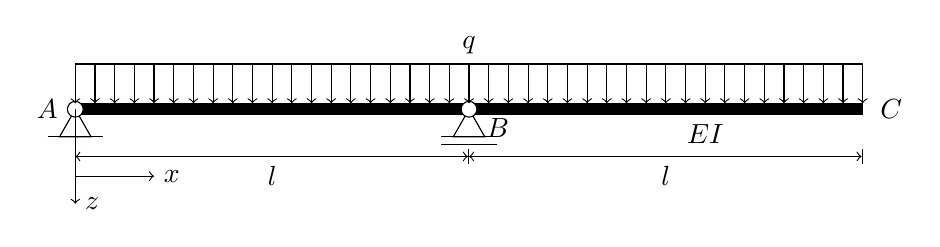
\begin{tikzpicture}
                \draw (-.2,-.25) -- (0,.1) -- (.2,-.25) -- cycle;
                \draw (-.35,-.25) -- (.35,-.25);
                \draw (4.8,-.25) -- (5,.1) -- (5.2,-.25) -- cycle;
                \draw (4.65,-.25) -- (5.35,-.25);
                \draw (4.65,-.35) -- (5.35,-.35);
                \fill (0,.025) rectangle (10,.175);
                \draw[fill=white] (0,.1) circle (1mm);
                \draw[fill=white] (5,.1) circle (1mm);
                \node[anchor=east] at (-.1,.1) {\(A\)};
                \node[anchor=north west] at (5.1,.1) {\(B\)};
                \draw[<->|] (0,-.5) -- (5,-.5) node[midway,below] {\(l\)};
                \draw[<->|] (5,-.5) -- (10,-.5) node[midway,below] {\(l\)};
                \draw[->] (0,.1) -- (0,-1.1) node[right] {\(z\)};
                \draw[->] (0,-.75) -- (1,-.75) node[right] {\(x\)};
                \node[anchor=north] at (8,.025) {\(EI\)};
                \node[anchor=west] at (10.1,.1) {\(C\)};
                \draw (0,.675) -- (10,.675) node[midway,above] {\(q\)};
                \foreach \i in {0,.25,...,10}
                {
                    \draw[->] (\i,.675) -- (\i,.175);
                }
            \end{tikzpicture}
        \end{center}
        Gegeben: \(EI\), \(q\), \(l\)
    \end{problem}

    \subsection*{Lösung}
    \begin{enumerate}
        \item Aus den Kräfte- und Momentengleichgewichten
        \begin{align*}
            \sum F_x: &\quad 0 = A_x,\\
            \sum F_z: &\quad 0 = -A_z - B_z + 2ql,\\
            \sum M_A: &\quad 0 = 2ql^2 - B_z l
        \end{align*}
        folgt für die Lagerreaktionen
        \[
            A_x = 0, \quad A_z = 0, \quad B_z = 2ql.
        \]
        \item Wir teilen den Träger in einen Bereich links (Index \(1\), \(0 \le x \le l\)) und in einem Bereich rechts (Index \(2\), \(l \le x \le 2l\)) vom Auflager in Punkt \(B\):
        \[
            M_1\parentheses*{x} = -\frac{1}{2}qx^2, \quad M_2\parentheses*{x} = -\frac{1}{2}q\parentheses*{2l - x}^2.
        \]
        Für die Biegelinien folgt durch Integration
        \begin{align*}
            w_1''\parentheses*{x}EI &= \frac{1}{2}qx^2, & w_2''\parentheses*{x}EI &= \frac{1}{2}qx^2 - 2qlx + 2ql^2,\\
            w_1'\parentheses*{x}EI &= \frac{1}{6}qx^3 + c_1, & w_1'\parentheses*{x}EI &= \frac{1}{6}qx^3 - qlx^2 + 2ql^2 x + c_3,\\
            w_1\parentheses*{x}EI &= \frac{1}{24}qx^4 + c_1 x + c_2, & w_2\parentheses*{x}EI &= \frac{1}{24}qx^4 - \frac{1}{3}qlx^3 + ql^2 x^2 + c_3 x + c_4.
        \end{align*}
        Mit den Rand- und Übergangsbedingungen
        \[
            w_1\parentheses*{0} = 0, \quad w_1\parentheses*{l} = 0, \quad w_2\parentheses*{l} = 0, \quad w_1'\parentheses*{l} = w_2'\parentheses*{l}
        \]
        folgt
        \[
            c_1 = -\frac{1}{24}ql^3, \quad c_2 = 0, \quad c_3 = -\frac{25}{4}ql^3, \quad c_4 = \frac{1}{3}ql^4
        \]
        und somit
        \begin{align*}
            w_1'\parentheses*{x}EI &= \frac{1}{6}qx^3 - \frac{1}{24}ql^3, & w_1'\parentheses*{x}EI &= \frac{1}{6}qx^3 - qlx^2 + 2ql^2 x - \frac{25}{4}ql^3,\\
            w_1\parentheses*{x}EI &= \frac{1}{24}qx^4 - \frac{1}{24}ql^3 x, & w_2\parentheses*{x}EI &= \frac{1}{24}qx^4 - \frac{1}{3}qlx^3 + ql^2 x^2 - \frac{25}{4}ql^3 x + \frac{1}{3}ql^4.
        \end{align*}
        Alternativ könnte die Biegelinie mit dem Superpositionsprinzip bestimmt werden.
        Hierzu würde das Problem in die Fälle 4 und 12 zerlegt.
        \item
        \[
            w_C = w_2\parentheses*{2l} = \frac{1}{4}\frac{ql^4}{EI}, \quad \alpha_C = w_C' = w_2'\parentheses*{2l} = \frac{7}{24}\frac{ql^3}{EI}.
        \]
        \item
        \[
            \alpha_A = w_A' = w_1'\parentheses*{0} 0 -\frac{1}{24}\frac{ql^3}{EI}, \quad \alpha_B = w_B' = w_1'\parentheses*{l} = \frac{1}{8}\frac{ql^3}{EI}.
        \]
    \end{enumerate}
\end{document}
